	\chapter{Experiments}
	In this section, several experiments to evaluate the effectiveness of our approach are presented. Selecting some approaches as baselines, our approach needs to be compared with these traditional ones and advanced ones to show its efficiency.
	\section{Dataset}
	The data prepared for baselines is also from the Stack Exchange data dump of 1st Sep. 2017 [1]. We collect 0.31 million duplicate question pairs and divide the duplicate question pairs into three groups that 80\% for training, 10\% for validation and 10\% for testing. The 80\% subset is mix up with 0.15 million non-duplicate pairs for training the CLSM model, the first 10\% subset is used for validation, and the last 10\% subset is used for the comparison process between our approach and the baselines.
	\section{Baseline Building}
	Two baselines are built below, which are Term Frequency-Inverse Document Frequency (TF-IDF) and The Word-n-Grams Letter-Trigram(CLSM).
	
	\subsection{TF-IDF}
	Term frequency-inverse document frequency(TF-IDF) is a well-known approach that predicts textual similarity with cosine distance [14]. This method is a statistical measure used to evaluate how important a word is to a document in a collection or corpus. Term Frequency measures how frequently a term occurs in a document. And Inverse Document Frequency measures how important a term is. The equation of the weight for term in a document is showed in Equation (4.1).\par
	\begin{normalsize}
		\begin{equation}
		Tf-Idf_{t,d} = Tf_{t,d} \cdot \log \frac{N}{df_t}
		\end{equation}
	\end{normalsize}
	For this baseline development, we use the same tokenizer as we have used in our approach to tokenize the same data, which is the training data for our DSSM. By calculating the term frequency and inverse document frequency for each word in the total word set, we can easily get the cosine similarity for a question pair.
	\subsection{Word-n-Grams and Letter-Trigram CLSM}
	
	From the literacy review, we found some excellent work that has been done in the more bottom level than the semantic level, such as the word level and letter level research [15]. Y. Shen, X. He, J. Gao, L. Deng, and G. Mesnil used the word-n-gram and letter-trigram model to build up a latent semantic model with pretty good results. The difference between the letter-trigram embedding with traditional word embedding is that every single word in the corpus needs to generate some letter trigrams. The letter trigrams represent all the sentences in the low dimensional vector space and then calculate the similarity between them. This method works very well in the letter and word levels, but the difficulty is that there is no well-developed letter trigram base. Nevertheless, this approach is also implemented. We trained this approach and compare the results with those of our DSSM approach in the experiment section. We generate a letter-trigram base from the corpus that we mined from Stack Overflow. Although the amount of letter trigram is not as great as we thought at first, we still apply the trigram base for letter embedding. 
\par
\begin{figure}[!h]
		\centering
		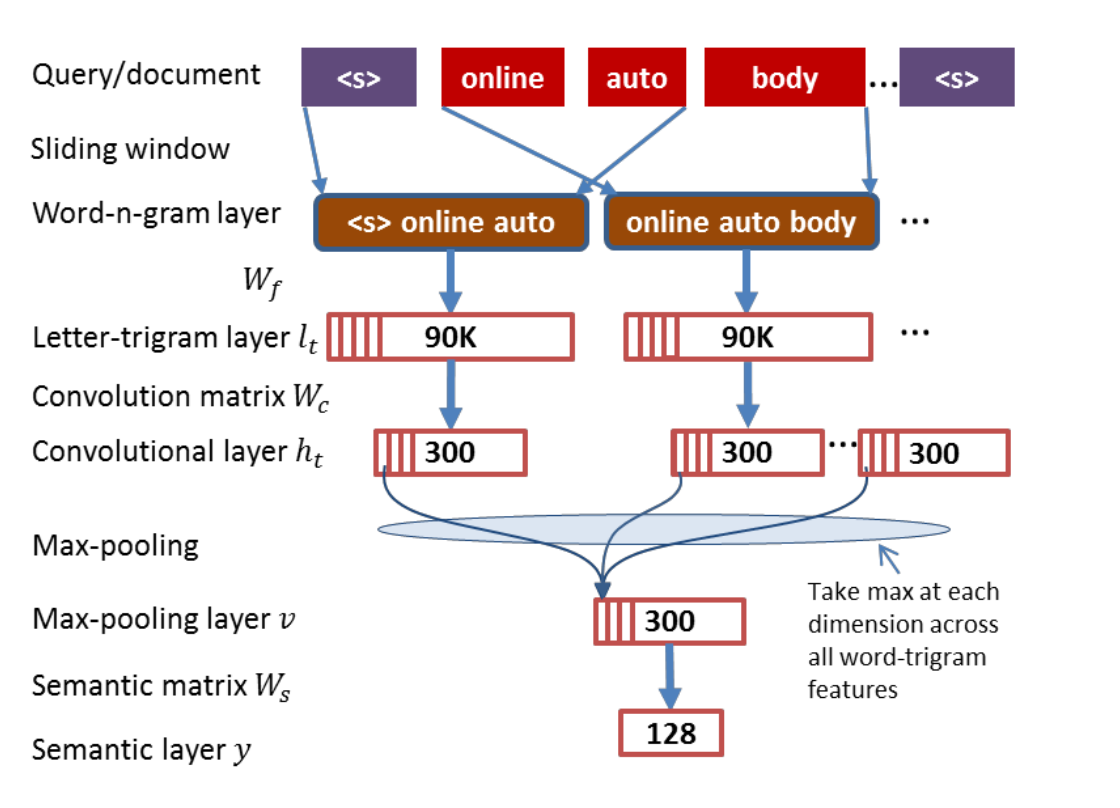
\includegraphics[width = 0.85\textwidth]{figures/wnglt.png}
		\caption{Model architecture of the Word-n-Grams and Letter-Trigram CLSM[15]}
	\end{figure}
The main architecture of the Word-n-Grams and Letter-Trigram convolutional latent similarity model is in Figure 4.1. It contains (1) the word-n-gram layer uses a contextual sliding window to get the word trigram sequence of the input sentence, (2) the letter-trigram layer embedding each word trigram into the embedding space, (3) the convolutional layer that combines the features for each word and both its neighbors. (4) the max-pooling layer transforms the word trigram features into a sentence level vector and (5) the final semantic layer that represents the semantic level vector of an input sentence.  \par
The input unit of this model includes a query, a positive sentence, and N negative sentences. And the output unit is a list of similarity, the sum of this list is 1 and represents the comparison of similarity between each sentence with the query. This baseline is used to evaluate the recommendating functionality of our model.

	
	\section{Evaluation Metrics}
	
	\subsection{Semantic Evaluation Metrics}
	According to some other excellent research [16, 17, 18, 19], some good evaluation metrics like accuracy, precision, recall rate and F1-score are the most widely used criterions in their experiments that can be applied to comparing the efficiency and accuracy of our approach and the baselines. Before illustrate how to calculate these criterions, there is a table for introducing some fundamental parameters.\par
	
	\begin{figure}[!h]
		\centering
		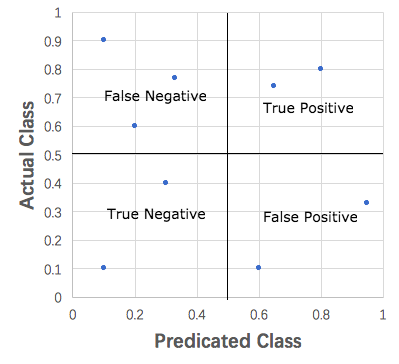
\includegraphics[width = 0.85\textwidth]{figures/class.png}
		\caption{Illustration: Relationship Between Predicted Class and Actual Class}
	\end{figure}
	Assume the method predict a question pair and get the similarity as a number in the range of 0 to 1, and from the label, we know the correct class is 0 or 1. In Figure 4.2, we divide 4 areas for different kinds of prediction. True Positives (TP) is predicted positive values and in the correct range according to the actual class. True Negatives (TN is predicted negative values and in the correct range according to the actual class. False Positives (FP) is predicted positive values and in the incorrect range according to the actual class. False Negatives (FN) is predicted negative values and in the incorrect range according to the actual class.
	\par
	Accuracy is simply a ratio of correctly predicted observation to the total observations, which is shown in the equation Equation (4.2).
	\begin{normalsize}
		\begin{equation}
		Accuracy =  \frac{TP+TN}{TP+FP+TN+FN}
		\end{equation}
	\end{normalsize}
	\par
	Precision is the ratio of correctly predicted positive observations to the total predicted positive observations, which is shown in the equation Equation (4.3).
	\begin{normalsize}
		\begin{equation}
		Precision =  \frac{TP}{TP+FP}
		\end{equation}
	\end{normalsize}
	\par
	Recall is the ratio of correctly predicted positive observations to the all observations in actual class, which is shown in the equation Equation (4.4).
	\begin{normalsize}
		\begin{equation}
		Recall =  \frac{TP}{TP+FN}
		\end{equation}
	\end{normalsize}
	\par
	F1 Score is the weighted average of Precision and Recall. Therefore, this score takes both false positives and false negatives into account, which is shown in the equation Equation (4.5).
	\begin{normalsize}
		\begin{equation}
		F1 =  \frac{2*Precision*Recall}{Precision+Recall}
		\end{equation}
	\end{normalsize}
	
	\subsection{Retrieval Evaluation Metrics}
	According to the existing research [20], we can use the Precision@k (pre@k) and Mean Average Precision (MAP) as evaluation metrics. Given a question pair as input, we have a query and its Ground Truth (GT). Simply evaluate the performance of our approach by calculating the metrics above. Precision@k determined by the most k relevant question of the query and the position of the Ground Truth. Mean Average Precision is the average value of all the testing queries.\par	
	
	\section{Evaluation}
	Some research problems related to the efficiency and functionality of our approach will be discussed and answered in this section.
	\subsection{Semantic Similarity Evaluation}
	{\bf Question1: How much advantages the new approach have compared with the traditional approaches in the semantic similarity field?}
	\par
	\begin{table}[!h]
		\centering
		\label{tab:table6}
		\scriptsize
		\begin{tabular}{|p{2.5cm} p{1.9cm}|p{1.9cm}|p{1.9cm}|p{1.9cm}|p{1.9cm}|}
			\hline    
			& & Accuracy & Precision & Recall & F1 Score \\
			\hline
			Baseline1& TF-IDF & 0.4070  &0.9049 &0.1555 &0.2654   \\
			\hline
			{\scriptsize Our Approach}& DSSM & 0.8026  & 1.0 & 0.8026 & 0.8904\\
			\hline    
			
		\end{tabular} 
		\caption{Overall comparison}
	\end{table}	
	Our semantic similarity model is based on the deep learning technique and uses word embedding to calculate the semantic similarity between two question titles, which is totally different with the traditional TF-IDF approach. And the comparison between these two approaches is in Table 4.1. As we can see, our approach has achieved a tremendous progress on the accuracy of predicting the semantic similarity. Respectively, our deep semantic similarity mode outperforms the baseline in several important criterions.
	\subsection{Retrieval Evaluation}
	{\bf Question2: How much advantages the new approach have compared with the current deep learning approaches in the information retrieval field?}
	The Table 4.2 shows the comparison between the Word-n-Gram and Letter-Trigram CLSM baseline and our approach. 
	\begin{table}[!h]
		\centering
		\label{tab:table7}
		\scriptsize
		\begin{tabular}{|p{2.5cm} p{1.9cm}|p{1.9cm}|p{1.9cm}|p{1.9cm}|p{1.9cm}|}
			\hline    
			& & Pre@1 & Pre@5 & Pre@10 & MAP \\
			\hline
			Baseline2& TF-IDF &  0.25 & 0.36& 0.42 & 0.31   \\
			\hline
			{\scriptsize Our Approach}& DSSM &  0.30 & 0.46 & 0.59 & 0.38 \\
			\hline    
		\end{tabular} 
		\caption{Overall comparison}
	\end{table}	
	All the Pre@K metrics of our approach are higher than those of the baseline2, But our approach does not far more better than the baseline. Because the data we used to train our deep semantic similarity model is the duplicate pairs manually marked by experts of Stack Overflow community, there are many other highly similar questions are still not marked. 
	\par
	In addition, our mode is a binary classification model, so it basically divides all the questions into two types, which are duplicate and non-duplicate. However, some non-duplicate question pairs generated for training are not totally without relation, which means some questions that recommended by our approach should be very similar to the query, but they are not marked duplicate. 
	\par
	The results confirm us that our deep semantic similarity model is effective in the Information retrieval area. Generally, a user always needs to get a large number of relative posts by the recommendation system, and our approach is better than the baseline2 when they both recommending a large number of posts.
	
	\subsection{Cross-lingual Question Retrieval Comparison}
	{\bf Question3: How does our approach performance in the cross-lingual question retrieval field?}
To answer this question, we randomly take a thousand Russian Posts from Russian Stack Overflow, which own a lower number of answers than others. These Russian posts are considered as query input, and we adopt google translate here to bridge the lingual gap. A black-box testing has been made by a lot of people to find out the efficiency and accuracy of our approach in the cross-lingual area. We collect all the recommendation posts generated by our approach, all the recommendation posts generated by the baseline2 and the recommendation posts generated by the Stack Overflow Search Engine. These three groups of recommendation posts are evaluated manually by volunteers to determine how good our approach is. And the results are very heuristic for us to improve our approach. 
\par
Our approach is better in some cases. There are some examples in Figure 4.3.
\begin{figure}[!h]
	\centering
	\subfigure[Recommendation 1 : From our approach]{\label{fig:a}
		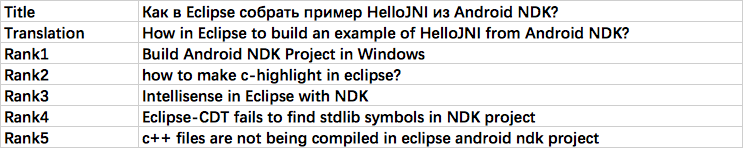
\includegraphics[width = 0.90\textwidth]{figures/exam1.png}
	}
	\subfigure[Recommendation 1 : From Baseline2 ]{\label{fig:a}
		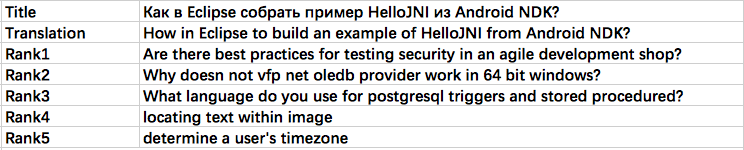
\includegraphics[width = 0.90\textwidth]{figures/exam2.png}
	}
	\caption{Examples of cross-lingual question retrieval}
	\label{fig}
\end{figure}
	
	